\subsection{Client- / Managerseitig}
\subsubsection{IRemoteLoggerClientConnection} \label{sec:IRemoteLoggerClientConnection}
\begin{wrapfigure}[6]{r}[0cm]{220px}
	\vspace{-20px} \hspace{5px}
	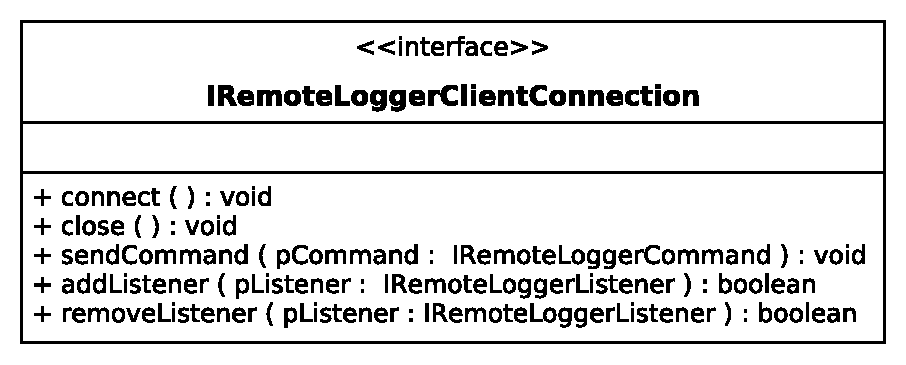
\includegraphics[width=215px]{../img/CD-IRemoteLoggerClientConnection.eps}
	\caption{Aufbau des Interfaces \glqq IRemoteLoggerClientConnection\grqq}
\end{wrapfigure}
\par Kapselt eine Verbindung zum Remote-Logger-Server. Der Verbindungsaufbau erfolgt in der \glqq connect()\grqq-Methode mit Hilfe der Java-eigenen Netzwerk-API. Dadurch erhält man einen InputStream und der ObjectInputStreamConsumer (siehe \prettyref{sec:ObjectInputStreamConsumer}) kann seine Arbeit beginnen.
\vspace{7px}
\begin{figure}[h] 
    \centering
	\begin{spacing}{0.75}
		\begin{javacode}[firstnumber=32]
clientSocket = new Socket(host, port);
streamConsumer = ObjectInputStreamConsumer.consume(clientSocket.getInputStream(), null, 
                                   this::_fireCheckPointReceived, this::_handleException);\end{javacode}
	\end{spacing}
	\caption{Initiieren der Verbindung zum Remote-Logger-Server am Remote-Logger-Client}
\end{figure}
\\
Falls vom Server ein \glqq IRemoteLoggerCheckPoint\grqq-Objekt empfangen wird, so wird die private Methode \glqq \_fireCheckPointReceived(...)\grqq\ aufgerufen. Diese iteriert die Liste der derzeit registrierten IRemoteLoggerListener (siehe \prettyref{sec:IRemoteLoggerListener}) und gibt den empfangenen IRemoteLoggerCheckPoint an jeden Listener weiter.
\par Ebenso ist es mit einer IRemoteLoggerClientConnection möglich, Kommandos an den Remote-Logger-Server zu senden (siehe \prettyref{sec:IRemoteLoggerCommand}).

\vspace{-5px}
\subsubsection{IRemoteLoggerListener} \label{sec:IRemoteLoggerListener}
\begin{wrapfigure}[5]{r}[0cm]{245px}
	\vspace{-17px} \hspace{5px}
	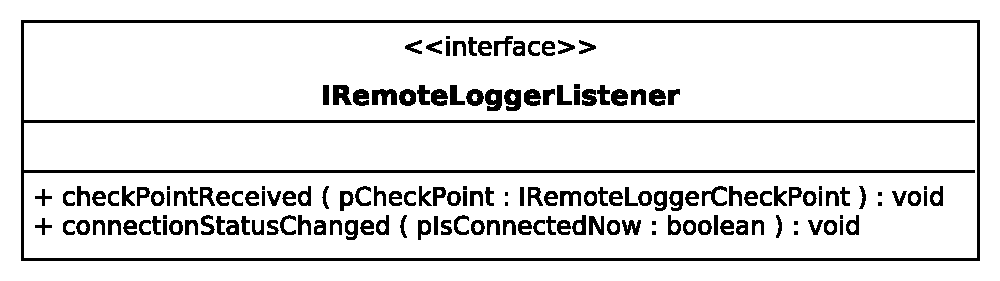
\includegraphics[width=240px]{../img/CD-IRemoteLoggerListener.eps}
	\caption{Aufbau des Interfaces \glqq IRemoteLoggerListener\grqq}
\end{wrapfigure}
\par Beschreibt einen Listener der zum einen aufgerufen wird, wenn sich der Status der Verbindung (Neue Verbindung, Verbindung getrennt) ändert und zum anderen wenn ein CheckPoint vom Remote-Logger-Server empfangen wurde.

\vspace{-5px}
\subsubsection{IRemoteLoggerClientConnectionManager}
\begin{wrapfigure}[7]{r}[0cm]{205px}
	\vspace{-20px} \hspace{5px}
	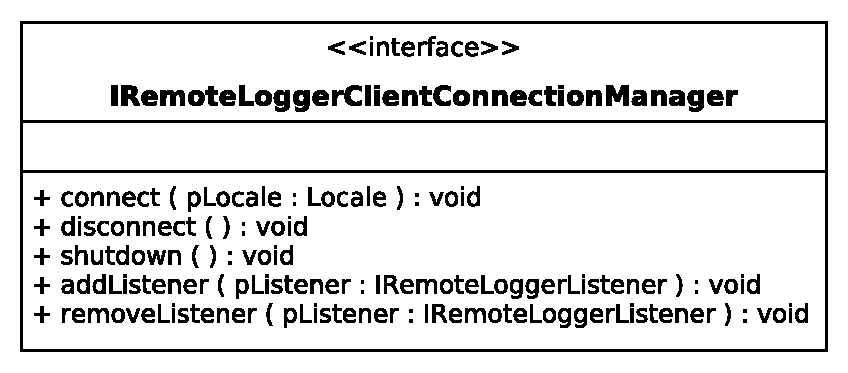
\includegraphics[width=200px]{../img/CD-IRemoteLoggerClientConnectionManager.eps}
	\caption{Aufbau des Interfaces \glqq IRemoteLoggerListener\grqq}
\end{wrapfigure}
\par Enthält und steuert eine IRemoteLoggerClientConnection (siehe \prettyref{sec:IRemoteLoggerClientConnection}). Dieser Manager bildet die zentrale Stelle der Verbindung zwischen Remote-Logger-Client und Remote-Logger-Server und sorgt dafür, dass die Verbindung gekapselt bleibt. Die \glqq connect(...)\grqq-Methode übernimmt einen zusätzlichen Parameter: Die Sprache der Verbindung (siehe \prettyref{sec:IRemoteLoggerCommand} - LanguageCommand).
\par Aufgrund des Sicherheitsaspekts ist das Senden von beliebigen Kommandos ab dieser Klasse von außen nicht mehr möglich. So sind Objekte an die Funktionalität des \glqq Connection-Managers\grqq\ gebunden und können keine eigenen Methoden hinzufügen. \\
Ein zentrales Registrieren von IRemoteLoggerListener ist hier ebenfalls möglich (siehe \prettyref{sec:IRemoteLoggerListener}). Das hat den Vorteil, dass beim Wechsel der IRemoteLoggerClientConnection-Instanz die Listener  automatisch von der alten Verbindung entfernt und zur neuen Verbindung hinzugefügt werden.

\newpage
\subsubsection{Graphical User Interface}
\begin{figure}[h] 
	\begin{center}
		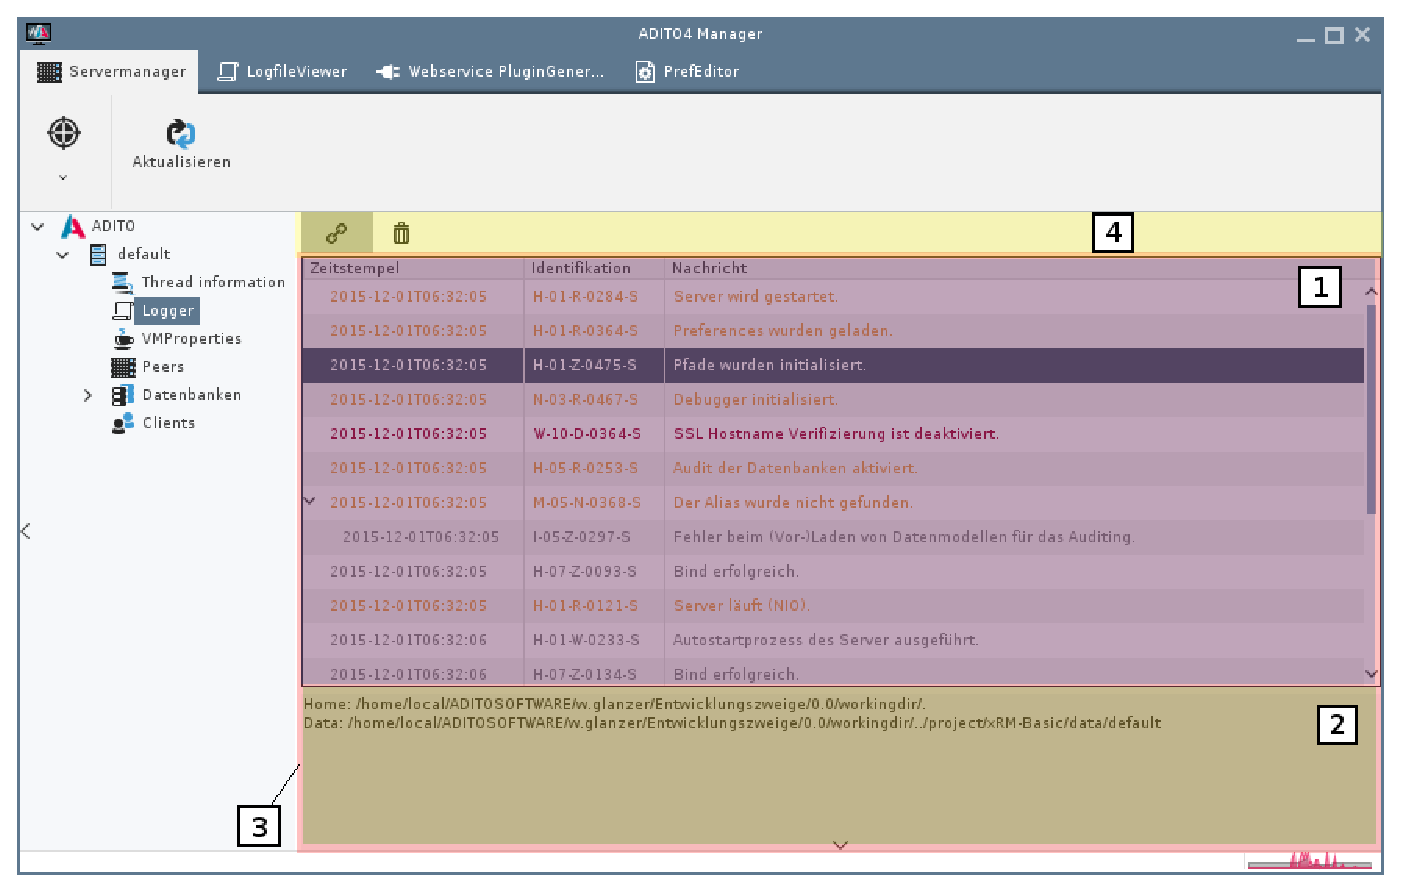
\includegraphics[width=0.9\textwidth]{../img/GUI-Manager.eps}
		\caption{Remote-Logger-Client innerhalb des ADITO4-Managers}
	\end{center}
\end{figure}
\par \textit{1. \underline{CheckPoint-Übersicht}} \vspace{-5px}
\par Die TreeTable entspricht der Hauptkomponente des Frames. Hier werden alle empfangenen CheckPoints farblich aufbereitet und dem Benutzer als Kombination von Baum und Tabelle präsentiert. \\
In der ersten Spalte befindet sich der Zeitstempel der besagt, zu welchem Zeitpunkt der CheckPoint aufgetreten ist. Die darauf folgende Spalte enthält den Identifikator, damit der jeweilige CheckPoint eindeutig im kompletten System zu identifizieren ist. Die hinter dem CheckPoint liegende, für den Benutzer lesbare Nachricht ist in der letzten Spalte platziert. Diese wird bereits in der richtigen Sprache vom Remote-Logger-Server geliefert.

\par \textit{2. \underline{Detailansicht}} \vspace{-5px}
\par In dieser Komponente (Instanz einer JTextArea) werden etwaige Details zu einem derzeit im Baum (1) selektierten CheckPoint dargestellt.

\par \textit{3. \underline{Container}} \vspace{-5px}
\par Als Container für o.g. Komponenten dient eine Abwandlung der JSplitPane. Allgemein bietet eine SplitPane Platz für zwei Komponenten, wobei sich mittels einem Trenner der Platz interaktiv durch den Benutzer aufteilen lässt. Im ADITO4-Manager wird nicht die originale JSplitPane benutzt, sondern die ADITO-spezifische \glqq OperaSplitpane\grqq, da diese die JSplitPane um eine Aufklappfunktion erweitert. Somit wird es dem Benutzer ermöglicht, die komplette zweite Komponente durch einen Button am unteren Rand unsichtbar zu schalten.

\par \textit{4. \underline{Toolbar}} \vspace{-5px}
\par Die Toolbar besitzt derzeit zwei Funktionen: Einerseits enthält sie eine Button, der bei Klick versucht die Verbindung zum Remote-Logger-Server aufzubauen, andererseits leert der zweite Button die Liste aller empfangenen CheckPoints, um somit eine verbesserte Übersichtlichkeit zu schaffen.